\section{ByteNet}
\label{sec:theory:bytenet}

The ByteNet model is an alternative approach to neural machine translation, it specifically focuses on having linear computational complexity, having a resolution preserving encoding, and be a character-level translation model \cite{bytenet}. This is somewhat different from existing popular models such as the Sutskever 2014 model \cite{sutskever-2014-nmt} and the attention based Bahdanau 2015 model \cite{bahdanau-2015-nmt}.

Note that the model presented here is a simplified version of the original ByteNet model \cite{bytenet}. First, there are no bags of characters, only individual characters are used as the sentence representation. Secondly, the sub-batch normalization in the decoder is replaced by layer normalization, besides being a simpler solution than sub-batch normalization this could also improve the model performance \cite{layer-normalization}. At last, the network has less weights a fewer layers than in the original ByteNet model.

\subsection{ByteNet Residual Block}

Before explaining the full ByteNet network, a central component of the ByteNet model called the \textit{ByteNet residual block} needs to be explained first. There are two variations of this an \textit{Encoder Residual Block}, and a \textit{Decoder Residual Block}. First the encoder version is explained and then some slight alterations of this will turn it into the decoder version. For a visual representation see Figure \ref{fig:bytenet:residual-block}.

\begin{figure}[h]
    \centering
    \begin{subfigure}[b]{0.45\textwidth}
        \centering
        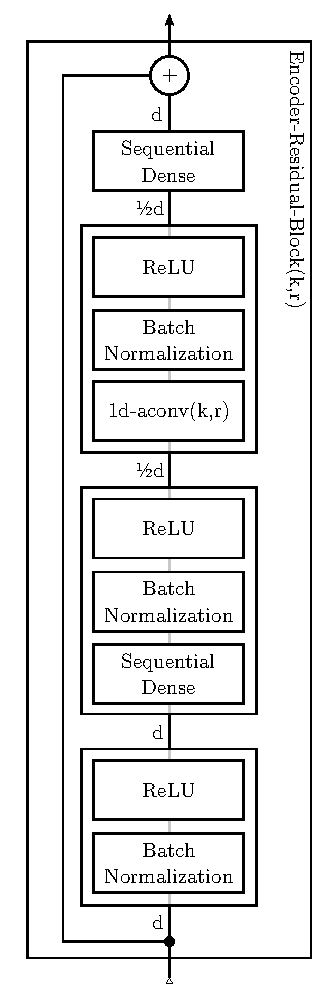
\includegraphics[scale=1]{theory/bytenet-residual-block.pdf}
        \caption{Residual Block used in encoder.}
    \end{subfigure}
    ~ %
    \begin{subfigure}[b]{0.45\textwidth}
        \centering
        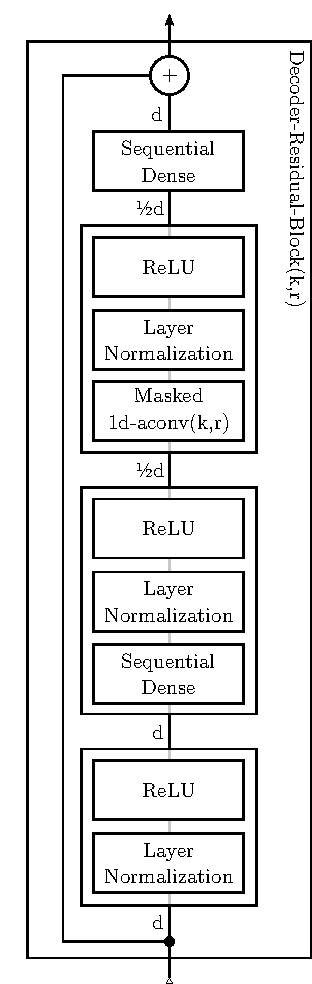
\includegraphics[scale=1]{theory/bytenet-residual-block-causal.pdf}
        \caption{Residual Block used in decoder.}
    \end{subfigure}
    \caption{The residual blocks used in the ByteNet model. The blocks are denoted by Encoder-Residual-Block$(k,r)$ and Decoder-Residual-Block$(k,r)$, where $k$ is the kernel width and $r$ is the dilation rate.}
    \label{fig:bytenet:residual-block}
\end{figure}

\subsubsection{Encoder Residual Block}

The \textit{ByteNet residual block} is at its core a dilated convolution, but adds upon this many of the ideas presented in section \ref{sec:convergence}. The entire block is a \textit{residual layer}, meaning that that the input is added to the final output of the transformation function $\mathcal{F}$. The transformation can be logically grouped into a set of sub-blocks, a normalization block, a dimensional reduction block, a dilated convolution block, and finally a dimensional restoration block.

The normalization block consists of batch normalization and a ReLU activation. For this to make sense there must be some parameters before the activation such that the network can control the ReLU. This will either be an embedding lookup or another \textit{residual block}.

The dimensional reduction block reduces the dimensionality of the dataset from $d$ dimensions to $\frac{1}{2}d$ dimensions. This is done through the usual dense layer, batch normalization, and ReLU activation block sequence. Note that the input is a sequence of vectors, a vector for each character, thus the dense matrix multiplication is performed on each vector in the sequence. This can also be described as a normal convolution with a kernel width of 1.

\afterpage{\clearpage}

The dilated convolution block depends on two parameters (or 3 if dimension size $d$ is included), the kernel width $k$ and the dilation rate $r$. ByteNet specifies a specific structure for these parameters, but these choices only make sense from the full network perspective, thus they will be discussed later. Besides being a dilated convolution the sub-block is quite normal, as it also performs a batch normalization and ReLU activation. The convolution also maintains the dimensionality, which at this point is $\frac{1}{2}d$.

For the \textit{residual layer} to make sense, the output dimension must be equal to the input dimension, thus the final sub-block is just a dense layer that transforms from $\frac{1}{2}d$ dimensions to $d$ dimensions. This sub-block does not contain either a batch normalization, or a ReLU activation. Though these are implicitly performed if another \textit{residual block} follows.

\todo[inline]{add parameter calculations}
\begin{equation}
\frac{k}{4} d_{enc}^2 + \frac{1}{2} d_{enc}^2 + \frac{1}{2} d_{enc}^2 = \left(\frac{k}{4} + 1\right) d_{enc}^2
\end{equation}


\subsubsection{Decoder Residual Block}

The decoder is very similar to the encoder, the differences exist such that the decoder can't look into the future of the target sequence. If the decoder was allowed to look into the future it would be impossible to perform inference, when the target sequence is unknown. To prevent future inspection two changes are made‚ the dilated convolution is masked, and batch normalization is replaced with layer normalization.

Masking the convolution means that only the part of the convolution kernel that looks at the past is preserved. This is equivalent to fixing the right side (the future side) of the preserved kernel to zero.

\todo[inline]{add parameter calculations, remember $d_{dec} = 2 d_{enc}$.}

\begin{equation}
\frac{\frac{k-1}{2} + 1}{4} d_{dec}^2 + \frac{1}{2} d_{dec}^2 + \frac{1}{2} d_{dec}^2 = \left(\frac{k + 1}{8} + 1\right) d_{dec}^2
\end{equation}


\subsection{Hierarchical Dilated Convolution}
\label{sec:theory:bytenet:hierarchical-dilated-convolution}

Each \textit{ByteNet Residual Block} can conceptually be seen as just a modified dilated convolution. This conceptual model is useful for understanding the main trick that makes \textit{ByteNet} so powerful, \textit{Hierarchical Dilated Convolution}.

The idea behind \textit{Hierarchical Dilated Convolution} is that by exponentially increasing the dilation rate in stacked dilated convolution layers, the effective kernel width will exponentially increase for each layer, while the amount of weight in the kernel only increases linearly. The encoder part (bottom half) of figure \ref{fig:bytenet:simplified-hdc} helps to understand this idea in detail.

\begin{figure}[h]
    \centering
    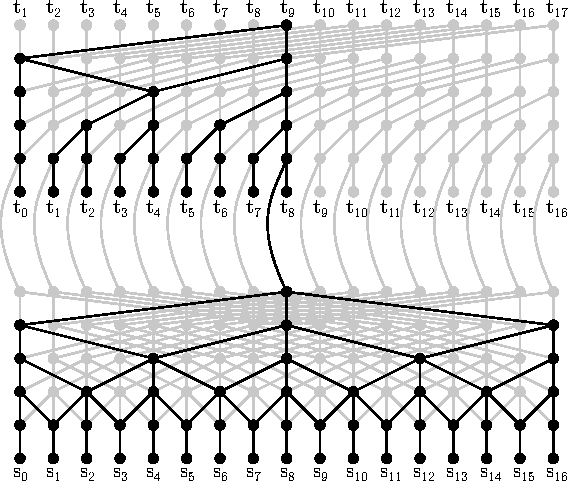
\includegraphics[scale=1]{theory/bytenet-hierarchical-dialted-convolution-enc-dec.pdf}
    \caption{A simplified version of the ByteNet model, showing the interaction between the decoder and encoder.}
    \label{fig:bytenet:simplified-hdc}
\end{figure}

Let the dilation rate for the encoding layers $\ell \in [1, L_{enc}]$ be denoted $r_\ell$, the exponential increasing dilation rate used in the ByteNet model is then $r_\ell = 2^{\ell - 1}$. The top layer $(L_{enc})$ will thus have a width of $(k-1) 2^{L_{enc} -1} + 1$. The effective total width is slightly larger because the layer below has a width of $(k-1) 2^{L_{enc} - 2} + 1$. This pattern continues down to the first layer, resulting in an effective total width of:
\begin{equation}
\sum_{\ell = 1}^{L_{enc}} (k - 1) 2^{\ell-1} + 1 = (k - 1) (2^{L_{enc}} - 1) + 1
\end{equation}
The kernel size is however $k \times d$ for all layers, thus the total amount of weights is:
\begin{equation}
\sum_{\ell = 1}^{L_{enc}} k d = L_{enc} k d
\end{equation}

In the original ByteNet model they use 5 dilated convolution layers, each with a kernel width of $5$, this results in an effective kernel width of 125 characters (actually it is 373 character wide because they repeat the pattern 6 times) \todo{redo calculations}. Having a wide but computationally cheap kernel is extremely important for a character-based translation model such as ByteNet. In an attention-based translation model, such as the Bahdanau model \cite{bahdanau-2015-nmt} the width is in theory arbitrarily wide (though in practice very wide attention mechanisms works poorly), however as discussed previously this approach causes a quadratic computational complexity (section \ref{sec:theory:sequential:bahdanau}). By \textit{hierarchical dilated convolution} ByteNet manages to keep the complexity linear, while still having a very wide kernel. In practice sentences have a limited length and thus a hierarchical dilated convolution approach can be comparable to an attention approach. In the WMT 2014 en-de dataset, the longest sentences are 400 characters wide (Figure \ref{fig:bytenet:wmt-deen-density}).

\begin{figure}[h]
    \centering
    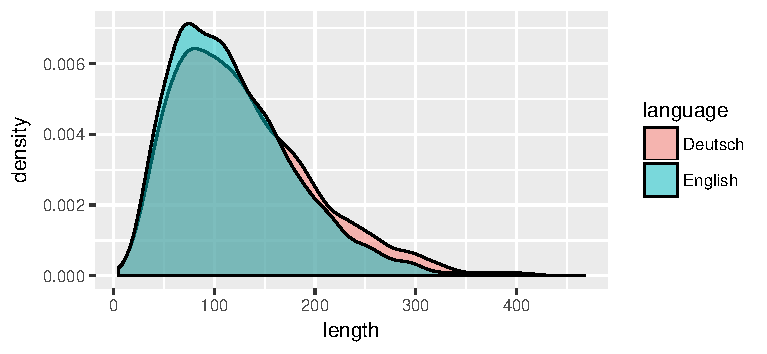
\includegraphics[scale=1]{theory/wmt-deen-density.pdf}
    \caption{Density estimate of the sentence length in the WMT 2014 en-de dataset.}
    \label{fig:bytenet:wmt-deen-density}
\end{figure}

\subsection{The Network}

The full \textit{ByteNet} model combines the \textit{Residual Blocks} with the \textit{Hierarchical Dilated Convolution} as discussed earlier. The \textit{Hierarchical Dilated Convolution} pattern is then repeated 3 times for both the encoder and decoder, as visualized in figure \ref{fig:bytenet:network}.

The input to the encoder is the source sequences mapped using an embedding matrix. The input to the decoder is the encoded sequence concatenated with the previous target prediction. This target prediction is then also mapped using a different embedding matrix. Note in particular that because the encoded vector is concatenated with the target sequence vector, the internal dimensionality of the decoder is twice that of the encoder. The decoded output is finally projected using a dense layer such the output has vocabulary sized dimensionality. After this, a softmax is used to transform the output into the probability domain.

An interesting effect of this network is that all layers are invariant to adding a bias term, as well as the $\gamma$ term in the normalization. The encoder embedding and encoder layers are invariant because of batch normalization. The decoder embedding and decoder layers are invariant because of layer normalization. The final dense layer is invariant because of the following softmax.

\begin{figure}[h]
    \centering
    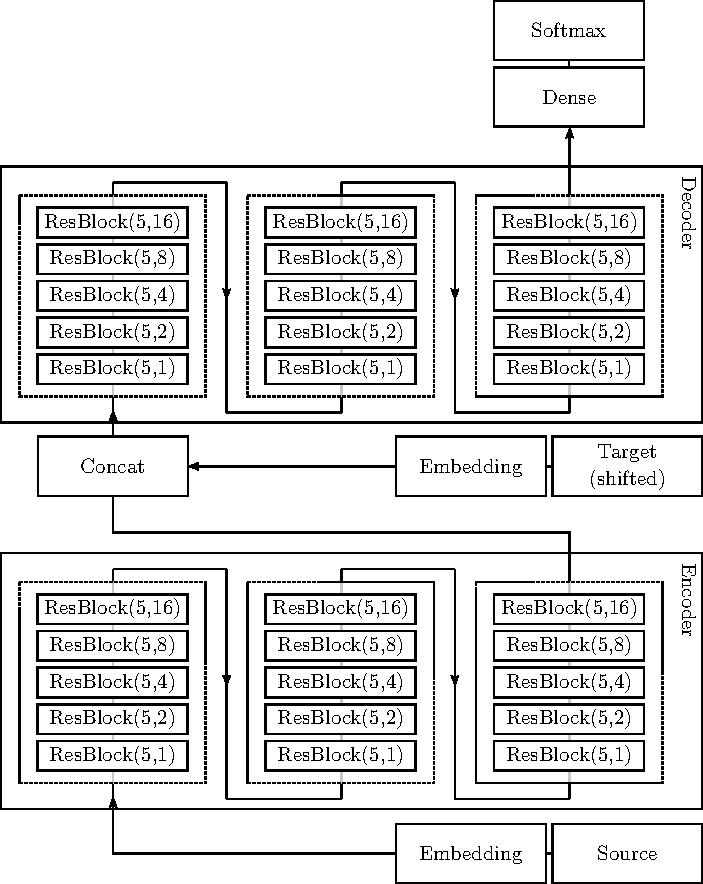
\includegraphics[scale=1]{theory/bytenet-network.pdf}
    \caption{The training network for the ByteNet Model, where the shifted target sequence is feed into the network. In the inference network, the shifted target sequence is replaced by the $\mathrm{argmax}(\cdot)$ of the softmax output. ResBlock$(k, r)$ in the encoder refers to the Encoder-Residual-Block$(k, r)$, in the decoder it refers to Decoder-Residual-Block$(k, r)$.}
    \label{fig:bytenet:network}
\end{figure}

\subsubsection{Training versus Inference}
The ByteNet model actually uses a different network for training than it does for inference. This is not strictly necessary, as one could use the same network for both training and interference like in an FFNN, however for sequential models the optimization can often converge faster if the target sequence is feed into the model.

Feeding the target sequence to the network is an optimization trick that may seem counter-intuitive at first. The idea is that because the prediction of the current character depends on the prediction of the previous characters ($\mathbf{y}_t = f(\mathbf{x}_{1:|S|}, \mathbf{y}_{1:t-1})$), then instead of letting the prediction cascade, which will also cause prediction errors to cascade, $\mathbf{y}_{1:t-1}$ is replaced with the known target sequence such that $\mathbf{y}_t = f(\mathbf{x}_{1:|S|}, \mathbf{t}_{1:t-1})$.

This trick also has the added benefit that training can be parallelized over target sentence and not just the observations and source sentence. 

\todo[inline]{There are some indications of this being suboptimal \url{https://arxiv.org/abs/1506.03099}}
